\problemname{Portaler}

Det nya företaget Sveriges Portaltrafik vill revolutionera hur svenska
pendlare tar sig runt i landet. Företaget har lagt fram
ett banbrytande förslag på hur ett portalsystem ska byggas i Sverige, för
att ersätta tåg, flyg och busstrafik med bränslesnåla portaler. Regeringen
har nu fått i uppdrag att granska förslaget i detalj, och vädjar till
svenska elitprogrammerare om hjälp. Det är här du kommer in i bilden.

Du har fått ta del av en ritning av portalsystemet för att analysera det.
Portalsystemet består av $N$ portaler utplacerade på olika platser i landet. Varje portal $a$
har en viss destinationsportal $b$. Det betyder att varje gång man går in i $a$ så kommer man
ut ur $b$. Notera att man inte nödvändigtvis kommer tillbaka till $a$ när man går in i $b$.
Sveriges Portaltrafiks nya idé är att genom att låta resenärer gå
i en portal och sedan upprepade gånger gå in i portalen man dyker upp vid så kommer man snabbt
kunna ta sig runt i landet.

Regeringen vill nu veta för ett antal givna start- och slutportaler $a$ och $b$
hur många gånger man behöver gå in i portalen man dyker upp vid för att ta sig från $a$ till
$b$ -- eller om det ens är möjligt. För varje sådan förfrågning ska du svara med antalet
gånger man behöver gå in i portalerna för att ta sig från $a$ till $b$. Om det är omöjligt
så ska du svara $-1$.

Hjälp regeringen!

\section*{Input}

På första raden i indata står heltalet $N$, antalet portaler som kommer att placeras ut i landet.
Sedan följer $N$ rader med tal $1 \le d_i \le N$ som beskriver att portalen på rad $i$ leder till portal $d_i$.
Portalerna är ett-indexerade (den lägsta har nummer 1, den högsta har nummer $N$), och kommer i ordning från $1$ till $N$ i indata.

Sedan följer en rad med ett heltal $Q$, antalet förfrågningar som du måste svara på. Efter det
följer $Q$ rader med två heltal $1 \le s, e \le N$. Dessa tal beskriver nummer på en startportal $s$ och en
slutportal $e$, och ditt uppdrag är att svara på hur många gånger man behöver gå igenom portalerna
för att ta sig till $e$ när man börjar vid $s$. För varje förfrågan gäller $s \neq e$.

\section*{Output}
Du ska skriva ut $Q$ rader, ett tal per förfrågan: antalet gånger man behöver gå
igenom portalerna för att ta sig från den givna startportalen till
slutportalen. Om det är omöjligt så skriver du ut $-1$. Skriv ut svaret
för varje förfrågan på en separat rad.

\section*{Förklaring av exempel}

\begin{figure}[ht!]
\centering
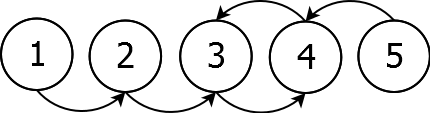
\includegraphics[width=0.4\textwidth]{portaler.png}
\caption{En illustration av Sample Input 1.}
\label{overflow}
\end{figure}

Nätverket i exempelfallet ser ut som i figuren. Vi får tre stycken förfrågningar. Den första
undrar hur många gånger vi behöver gå in i portalerna när vi börjar vid $1$ och vill hamna
vid $2$. Eftersom man direkt hamnar vid $2$ när man går in i $1$ så är svaret $1$. För att
ta sig från $1$ till $4$ så krävs tre hopp. För den sista förfrågan är svaret $-1$,
eftersom vi aldrig kan ta oss från $2$ till $5$, oavsett hur länge vi går igenom portalerna.

\section*{Poängsättning}
Din lösning kommer att testas på en mängd testfallsgrupper. För att få poäng för en grupp
så måste du klara alla testfall i gruppen.

\begin{tabular}{| l | l | l | l |}
\hline
Grupp & Poängvärde & Gränser & Övrigt\\ \hline
1     & 10         & $ 1 \le N \le 1\,000,\ 1 \le Q \le 1\,000$ & Det kommer alltid finnas en väg mellan start- och slutportalerna.\\ \hline
2     & 20         & $ 1 \le N \le 1\,000,\ 1 \le Q \le 1\,000$ &  \\ \hline
3     & 10         & $ 1 \le N \le 7\,000,\ 1 \le Q \le 120\,000$ & Det kommer alltid finnas en väg mellan start- och slutportalerna.\\ \hline
4     & 10         & $ 1 \le N \le 7\,000,\ 1 \le Q \le 120\,000$ &  \\ \hline
5     & 10         & $ 1 \le N \le 50\,000,\ 1 \le Q \le 70\,000$ & Det kommer alltid finnas en väg mellan start- och slutportalerna. Testfallen är också lite snällare än grupp 6.\\ \hline
6     & 30         & $ 1 \le N \le 50\,000,\ 1 \le Q \le 70\,000$ & Det kommer alltid finnas en väg mellan start- och slutportalerna. \\ \hline
7     & 10         & $ 1 \le N \le 50\,000,\ 1 \le Q \le 70\,000$ &  \\ \hline
\end{tabular}
